\subsection{Introduction}
The goal of this text is to give an overview of the geometry behind \'etale cohomology, in particular how Galois representations arise from \'etale cohomology of varieties over $\Q$

\section{Reminder on Schemes}
The basic building blocks of algebraic geometry are affine schemes. An affine scheme $\Spec(A)$ is a geometric object constructed out of the prime spectrum 
\[
  \Spec(A) = \{p \subseteq A \mid p \text{ prime ideal}\}
\]
of a commutative ring $A$. We would like to interpret the ring $A$ as the ring of functions on $\Spec(A)$, analogous to the ring 
$\Sh{O}(M) := \{f: M \to \R \mid f \text{ continuous}\}$
 for a manifold $M$. As a notational trick we write $f(p)$ for the image of $f$ under the quotient map $A \to A/p$. Note that the domain of a function $f$ depends on where it is evalued! The function $f \in A$ sends a point $p \in \Spec(A)$ to $f(p) = \overline{p} \in A/p$.  However, we will often consider schemes over a field, which are schemes equipped with a morphism $X \to \Spec(k)$, $k$ a field. This field will then play the role of $\R$ as in the example of manifolds. We equip $\Spec(A)$ with the Zariski topology, which has a basis given by sets of the form 
\begin{align*}
  D_f &= \{ p \in \Spec(A) \mid (f) \not \subseteq p \} \\
      &= \{ p \in \Spec(A) \mid f(p) \neq 0\} .
\end{align*}
\begin{definition}
    The \textit{Zariski topology} on $\Spec(A)$ consists of open sets of the form $D_I = \{ p \in \Spec(A) \mid I \not \subset (p)\}$ where $I \subseteq A$ is an ideal. The closed sets are of the form
    \begin{align*}
        V_I &= \{ p \in \Spec(A) \mid (f) \subseteq p \} \\
            &= \{ p \in \Spec(A) \mid f(p) = 0\},
    \end{align*}
    the \textit{vanishing set} or \textit{zero locus} of $f$. 
\end{definition}

Since $f(p) \neq 0$ for all $p \in D_f$, we view the the ring $A[1/f]$ as the ring of rational functions defined on $D_f$. It consists of elements of the form 
\[
  \biggl\{ \frac{g}{f^k} \mid g \in A, k \in \N \biggr\}.
\]
The assingment $D_f \to A[1/f]$ extends to a sheaf $\Sh{O}_{\Spec{A}}: \Spec(A) \to \mathsf{Ring}$, called the \textit{structure sheaf of $\Spec(A)$}. This sheaf is again in analogy with the sheaf We obtain a fully faithful functor
\[
\Spec : \text{CRing}^{op} \to LRS
\]
from the category of commutative rings to the category of locally ringed spaces. An affine schemes is a locally ringed space isomorphic to $\Spec(R)$ for some ring $R$. Basic examples of affine schemes arise from polynomial rings: scheme-theoretically, the zero locus of a polynomial $f \in k[x_1, \dots, x_n]$ is the spectrum $\Spec(k[x_1, \dots, x_n]/(f))$, for instance the parabola is the locally ringed space $\Spec(k[x,y]/(x^2-y))$.

\begin{definition}
  A \textit{scheme} is a locally ringed space $X$ such that there is a covering $\{U_i\}_{i \in I}$ of $X$ such that each $U_i$ is isomorphic to an affine scheme $\Spec(A_i)$ for some ring $A_i$.
\end{definition}

\section{Motivation for Cohomology}
One of the most important invariants of schemes is \'etale cohomology.  Cohomology is an important invariant in geometry and topology which associates to each space $X$ a sequence of abelian groups $H^i(X)$, $i \ge 0$, the so-called cohomology groups of $X$. For each map $f: X \to Y$ of spaces there are homomorphisms $f^*: H^i(Y) \to H^i(X)$. Moreover there are so called coboundary morphisms $\partial^i : H^i \to H^{i+1}$ for each $i \ge 0$.
\begin{definition}
    A \textit{cohomology theory} for
\end{definition}
We can deduce many interesting properties of spaces from their cohomology groups and the associated homomorphisms.

An important and intuitive cohomology is \textit{singular cohomology}. It provides a rigorous way for counting ``holes'' in a topological space.  For instance, the circle $S^1$ has 1 one-dimensional hole while the torus $T^2$ has 2. The sphere $S^2$ has 1 two-dimensional hole but no one-dimensional holes, in symbols 
\footnote{$\Z$ appears here because it is the free group on one generator.}
\begin{align*}
  H^1_{sing}(S^1) \simeq \Z,\quad &H^1_{sing}(T^2) \simeq \Z \oplus \Z,\\
  H^1_{sing}(S^2) \simeq  0,\quad &H^2_{sing}(S^2) \simeq \Z.
\end{align*}
One very general approach to cohomology is to use sheaves on a topological space as ``coefficients''. Sheaves consist of local data on a space that is glueable. A basic example consists of functions on a space: If we have an open cover $\{ U_i\}$ for a manifold $M$ and functions $f_i: M \to \R$ that agree on all intersections $U_i \cap U_j$ we may patch it together to a function $f: M \to \R$.
 For any space $X$ and any sheaf $\Sh{F}$ on $X$ we can define $H^i(X, \Sh{F})$. Many examples of cohomology theories turn out to stem from the cohomology of a particular sheaf. For example, if $X$ is a locally contractible space, the singular cohomology $H_{\text{sing}}^i(X)$ of $X$ is isomorphic to the sheaf cohomology $H^i(X, \Z_X)$ of the constant sheaf $\Z_X$ on $X$.

One of the main motivations for \'etale cohomology is that one would like a replacment for singular cohomology for schemes. There are a number of obstacles:
\begin{proposition}\label{scheme_contractible}
    An irreducible scheme is contractible.
\end{proposition}
\begin{proof}
  Define a map $f: X \times I \to X$  by $f(x,0) = x$ and $f(x,t) = \eta$ for $t > 0$. This is a contraction of $X$ onto the point $\eta$, so. the singular cohomology of $X$ is identically 0.
\end{proof}

\begin{proposition}
  $H^i(X, \Sh{F})$ is 0 for any sheaf on an irreducible topological space.
\end{proposition}
\begin{proof}
    See section TODO.
\end{proof}
This is a strong indication that the traditional tools of cohomology are inadequate to analyse the geometry of schemes.


\section{Fundamental groups}
Another important invariant of spaces is the fundamental group. The fundamental group of a pointed topological space $(X,x)$, denoted by $\pi_1(X,x)$ may be defined in two equivalent ways: Via homotopy classes of loops in $X$ based at $x$, or as the automorphism group of the fiber functor $F_x: Cov(X) \to Set$. From the first perspective, the fundamental group measures the connectivity of a space. The construction makes use of the unit interval. The unit interval $[0,1] \subset \R$ is not an algebraic set so the first definition does not have a natural formulation using only the notions of algebraic geometry. The second approach yields a theory strongly reminiscent of Galois theory. Grothendieck pioneered this approach in algebraic geometry.

\subsection{The fundamental group via paths}
    A loop with base point $x$ is a map $\gamma : [0,1] \to X$ such that $\gamma(0) = \gamma(1) = x$. The homotopy class of $\gamma $ is denoted by $[\gamma]$. Define a composition operation by concatenation: $[\gamma] \circ [\eta] = [\gamma \circ \eta]$, where $\gamma \circ \eta$ is defined to be the path 
    \[
      \gamma \circ \eta =
        \begin{cases}
            \ \eta(2x) \text{ for } x \in [0, \tfrac{1}{2}]\\
            \ \gamma(2x - 1) \text{ for } x \in [\tfrac{1}{2}, 1].
        \end{cases}
    \]
    It is clear that this construction yields a group structure on the set 
    \[
        \{\ [\gamma] \mid \gamma : [0,1] \to X , \gamma(0) = \gamma(1) = x \}
    \]
    of homotopy classes of loops at $x$.

\subsubsection{The monodromy action}

\begin{construction}[Covering spaces]
    Let $X$ be a topological space. A \textit{space over $X$ } is a topological space $Y$ together with a continuous map $Y \to X$. A morphis between two spaces $Y_1, Y_2$ over $X$ is a continuous map $f: Y_1 \to Y_2$ such that the diagram
    \[
    % https://q.uiver.app/?q=WzAsMyxbMCwwLCJZXzEiXSxbMiwwLCJZXzEiXSxbMSwxLCJYIl0sWzAsMSwiZiJdLFsxLDIsInBfMiJdLFswLDIsInBfMSIsMl1d
    \begin{tikzcd}
    	{Y_1} && {Y_1} \\
    	& X
    	\arrow["f", from=1-1, to=1-3]
    	\arrow["{p_2}", from=1-3, to=2-2]
    	\arrow["{p_1}"', from=1-1, to=2-2]
    \end{tikzcd}
    \]
    commutes. We obtain the category $\Top/X$ of spaces over $X$.  A space $f: Y \to X$ over $X$ is called a local homeomorphism if for any point $y \in Y$ there is a neighborhood $U$ of $x$ such that the preimage $f^{-1}(U)$ is homeomorphic to a disjoint union of the open sets $f^{-1}(U) \cong \coprod U_i$ such that each $U_i$ gets mapped to $U$ homeomorphically under $f|_{U_i}$. Surjective local homeomorphisms over a space $X$ are also called \textit{covering spaces of $X$} or simply \textit{coverings}.  Let $f: Y \to X$ be a surjective local homeomorphism.  A trivial covering is one of the form $p: \coprod X \to X$, where $p$ restricts to the identity on each component. Using this terminology one can also say that a covering is a \textit{locally trivial local homemorphism}. 
\end{construction}

\begin{lemma}[Path-lifting property of covering spaces]
  Let $p: Y \to X$ be a cover, $y \in Y$ and $x = p(y) \in X$. 
  \begin{enumerate}
    \item If $f: [0,1] \to X$ is a path in $X$ with $f(0) = x$, then there is a unique path $\tilde{f}: [0,1] \to Y$ with $\tilde{f}(0) = y$ and $p \circ \tilde{f} = f$
    \item Assume we have a second path $g: [0,1] \to X$ homotopic to $f$ with the same endpoints. Then the unique lift $\tilde{g}$ of $g$ to $Y$ is homotopic to $\tilde{f}$ with the  same endpoints.
  \end{enumerate}
\end{lemma}
\begin{proof}
  See \cite{Szamuely}, Lemma 2.3.2.
\end{proof}
\begin{construction}(The monodromy action)
  Let $p(y)=x$ and let $\alpha \in \pi_1(X,x)$ be represented by a path $f: [0,1] \to X$. By the previous lemma, there is a unique lift $\tilde{f}$ with $\tilde{f}(0) = y$. Since $p \circ \tilde{f} = f$, we have $(p \circ \tilde{f})(1) = x$, so the fundamental group $\pi_1(X, x)$ acts on $F_x(Y)$. This action is called the \textit{monodromy action}.
\end{construction}

A $Y$-automorphism is defined to be an automorphism of $Y$ in $\Top/X$. Let $Cov(X)$ be the subcategory of $\Top/X$ consisting of covering spaces. For each point $x \in X$ there is a functor $F_x: Cov(X) \to \Set$, sending a covering $p: Y \to X$ to the set $\{y \in Y \mid p(y) = x\}$. Now define an automorphism of $F_x$ to be a natural transformation $\psi: F_x \to F_x$ with a two-sided inverse. The set $\text{Aut}(F_x)$ of automorphisms of $F_x$ carries the structure of a group by composition. Note that for a covering $Y$ of $X$ and an automorphism $\phi \in \text{Aut}(F_x)$, there is by definition a morphism $\phi(Y): F_x(Y) \to F_x(Y)$. We define $\pi_1(X,x)$ to be the automorphism group of $F_x$.

We would like to have a notion of fundamental group for schemes. As before, there are some obstacles:

\begin{itemize}
  \item  As we have seen in \ref{scheme_contractible}, any irreducible scheme $X$ is contractible. As every loop in an irreducible scheme is contractible, this implies that $\pi_1(X)$ is $0$. In a sense this means that the unit interval is not a suitable ``test space'' to probe varieties and schemes.
  \item There is no universal covering space.
        For instance, the algebra homomorphism given by $x^n \to x^n, k[x^n] \to k[x]$ corresponds to a map $x \to x^n, \mathbb{A}^1_k \to \mathbb{A}^1_k$. Depicted is the map from $\mathbb{A}^1_\C$ to $\mathbb{A}^1_\C$ for the case $n=2$

          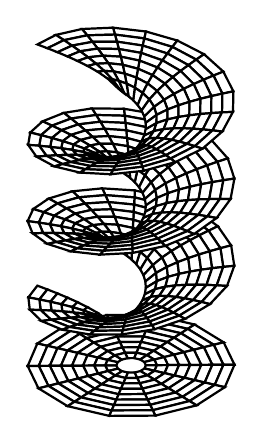
\begin{tikzpicture}[scale=2]
    \begin{axis}[
        axis lines=none,
        axis equal image,
        trig format plots=rad,
        z buffer=sort]
   \addplot3 [
        surf,
        domain=1:7,
        domain y=-pi:pi,
        samples=9,
        samples y=15,
        shader=flat,
        draw=black,
        fill=white
        ]
    ({x*cos(y)},{x*sin(y)},{-12});
   \addplot3 [
        surf,
        domain=1:7,
        samples=9,
        samples y=60,
        shader=flat,
        draw=black,
        fill=white,
        domain y=-3*pi:3*pi
        ]
    ({x*cos(y)},{x*sin(y)},{ln(x)+ y});
    \end{axis}
  \end{tikzpicture}



        This map \textit{should} be local homeomorphism, but this is false in the Zariski topology. There do not exist nonempty open subsets $V$ and $U$ such that $x \to x^n$ maps $V$ isomorphically onto $U$. The theory of \'etale coverings will give us a good notion of covering which we will use to define the analog of universal coverings
\end{itemize}

The \'etale topology will provide a solution for the problems we have with both cohomology and fundamental groups. The \'etale topology is not a topology in the classical sense, but a category equipped with a notion of covering (in the sense of point-set topology). The analog of open sets of a scheme $X$ will be so called \'etale morphisms $U \to X$. \'Etale morphisms are the natural analogs of local homeomorphisms in scheme theory, so they provide a finer topology than the Zarisiki topology, giving rise to a better sheaf theory. Furthermore, surjective \'etale morphisms share a lot of formal properties with covering spaces, allowing us to define the \'etale fundamental group $\pi_1^{\et}$.

\subsection{Overview}
We first develop the theory of \'etale maps and their Galois theory. This theory generalises classical Galois theory from fields to schemes and will allow us to define the fundamental group $\pi_1^{\et}(X)$ of a connected scheme $X$. Then we introduce the notion of site and define sheaves on sites as a direct generalisation of sheaves on a topological space. We then take a closer look at sheaves on the \'etale site of a scheme and study their cohomology.
\subsection{Prerequisites}
We assume aqcuaintance with the basics of category theory including limits and adjoint functors. We will make free use of results from algebra but will provide references wherever needed. We will also use basic notions of scheme theory.

%
\subsection{Interpretation of Cohomology}
Cohomology groups are not just of interest in their own right. In many cases, one can show that the cohomology classes $[\gamma] \in H^n(X, \Sh{A})$ correspond bijectively to some other kind of geometrical construction involving $X$.

For instance, when $p:Z \to B$ is a map of topological spaces and $\Sh{G}$  is a sheaf of subgroups of $Aut_B(Z)$, one can define a notion of “twist of $p$ with structure sheaf $\Sh{G}$”. One obtains the bijection
\begin{align}
            \left\{ \parbox[c]{1.1in}{\centering
                       Isomorphism classes of twists of $p$
                       with structure sheaf $\Sh{G}$}
            \right\}
            \stackrel{\sim}{\to}
            \parbox[c]{0.5in}{\centering
                       $H^1(B, \Sh{G})$}
\end{align}

There is also a bijection
\begin{align}
            \left\{ \parbox[c]{1.1in}{\centering
              Isomorphism classes of vector bundles of rank $n$ with basis $B$}
            \right\}
            \stackrel{\sim}{\to}
            \parbox[c]{0.5in}{\centering
            $H^1(B, GL_{n,B})$}
\end{align}
and in particular
\begin{align}
            \left\{ \parbox[c]{1.1in}{\centering
            Isomorphism classes of line bundles with basis $B$}
            \right\}
            \stackrel{\sim}{\to}
            \parbox[c]{0.5in}{\centering
                $H^1(B, \Ring(O)_B^\times)$}
\end{align}

%\subimport{introduction/}{mobius.tex}